\documentclass[12pt,a4paper]{article}
\usepackage[margin=.5in]{geometry}
\usepackage[utf8]{inputenc}
\usepackage[IL2]{fontenc}
\usepackage[czech]{babel}
\usepackage{microtype}
\usepackage{amssymb}
\usepackage{amsthm}
\usepackage{amsmath}
\usepackage{xcolor}
\usepackage{graphicx}

\usepackage[inline]{enumitem}

\newcommand{\R}{\mathbb{R}}

\DeclareMathOperator{\tg}{tg}
\DeclareMathOperator{\cotg}{cotg}

\setlist[enumerate]{label={(\alph*)},topsep=\smallskipamount,itemsep=\smallskipamount,parsep=0pt}
\setlist[itemize]{topsep=\smallskipamount,noitemsep}


\theoremstyle{definition}
\newtheorem{uloha}{Úloha}
\newtheorem*{bonus}{Bonus}

\pagestyle{empty}

\let\ee\expandafter

\def\vysld{}
\let\printvysl\relax
\let\printalphvysl\relax

\makeatletter
\def\vyslplain#1{\ee\ee\ee\gdef\ee\ee\ee\vysld\ee\ee\ee{\ee\vysld\ee\printvysl\ee{\the\c@uloha}{#1}}}
\let\vysl\vyslplain

\def\locvysl#1{\ee\gdef\ee\locvysld\ee{\locvysld\item #1}}
\let\lv\locvysl

\newenvironment{ulohav}{\begin{uloha}\gdef\locvysld{\begin{enumerate*}}}{\ee\vyslplain\ee{\locvysld\end{enumerate*}}\end{uloha}}

\makeatother

\begin{document}

\section*{Stereometrické polohy}

% totální vykrádačka stereometrické sbírky
% https://kag.upol.cz/data/upload/17/sbirka_uloh_stereometrie_140916(1).pdf

Ve všech úlohách značí $S_{XY}$ střed úsečky $XY$.


\begin{uloha}
Uvažme v prostoru tři roviny, kde žádné dvě z nich nejsou totožné. Vymyslete jejich všechny možné konfigurace (celkem pět), které se budou lišit v tom, jaké budou průniky dvojic rovin a/nebo jaký bude průnik všech tří dohromady.

Např. jednou možnou konfigurací je, že jsou všechny tři roviny navzájem rovnoběžné (tím pádem je průnik každých dvou prázdný a tím spíš i průnik všech tří dohromady).
\vysl{%
Možnosti jsou: \begin{enumerate*}[label={(\arabic*)}]
    \item všechny tři roviny rovnoběžné, \item dvě rovnoběžné a třetí s nimi různoběžná (ta se s nimi protíná ve dvou rovnoběžných přímkách, takže průnik všech je prázdný), \item každé dvě roviny jsou různoběžné, ale jejich průsečnice jsou rovnoběžné (takže průnik všech je prázdný), \item každé dvě roviny jsou různoběžné a jejich průsečnice splývají (takže průnik všech je přímka), \item každé dvě roviny jsou různoběžné a průsečnice jsou také různoběžné (potkávají se v jednom bodě, který je společným průnikem všech tří rovin).\end{enumerate*}
\[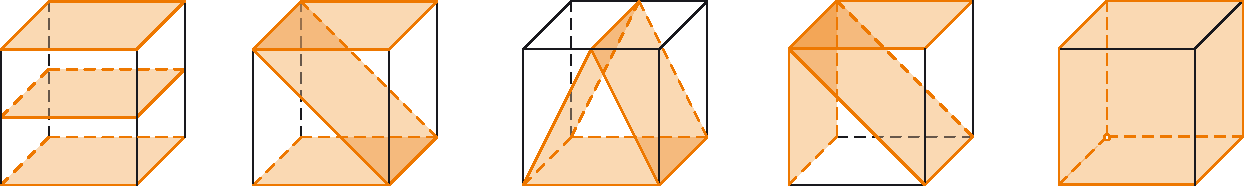
\includegraphics[scale=.8]{roviny_konfigurace.pdf}\]%
}
\end{uloha}

\let\vysl\vyslalph


\begin{ulohav}
Uvažme krychli $ABCDEFGH$.
Rozhodněte, zda jsou uvedené dvojice přímek rovno-, různo-, či mimoběžné: \begin{enumerate}
    \item $AS_{GH}$ a $S_{AB}D$, \lv{mimo}
    \item $AP$ a $BS_{CG}$, bod $P$ je střed stěny $CDGH$, \lv{různo}
    \item $AP$ a $S_{AE}S_{GH}$, bod $P$ je střed stěny $CDGH$, \lv{rovno}
    \item $AS_{GH}$ a $EC$, \lv{mimo}
    \item $S_{AB} S_{AD}$ a $FH$, \lv{rovno}
    \item $AH$ a $S_{BF}G$, \lv{mimo}
    \item $BD$ a $S_{BF}H$, \lv{různo}
    \item $BH$ a $S_{AE}S_{CG}$. \lv{různo}
\end{enumerate}
\end{ulohav}


\begin{uloha}
Uvažme opět krychli $ABCDEFGH$.
Rozhodněte o vzájemné poloze dvou rovin, v případě různoběžných rovin určete (konstrukčně) jejich průsečnici.
\begin{enumerate}
    \item $BFS_{AC}$, $HFS_{EH}$
    \item $AFH$, $BDG$
    \item $EFG$, $BCS_{AE}$
    \item $ABS_{DH}$, $S_{AB} S_{CG} S_{CH}$
    \item $ACE$, $AFH$
    \item $EGS_{BC}$, $BHF$
    \item $ABG$, $HFS_{AD}$
    \item $ABC$, $FHS_{AE}$
    \item $ABC$, $AFH$
\end{enumerate}%
\vyslplain{\[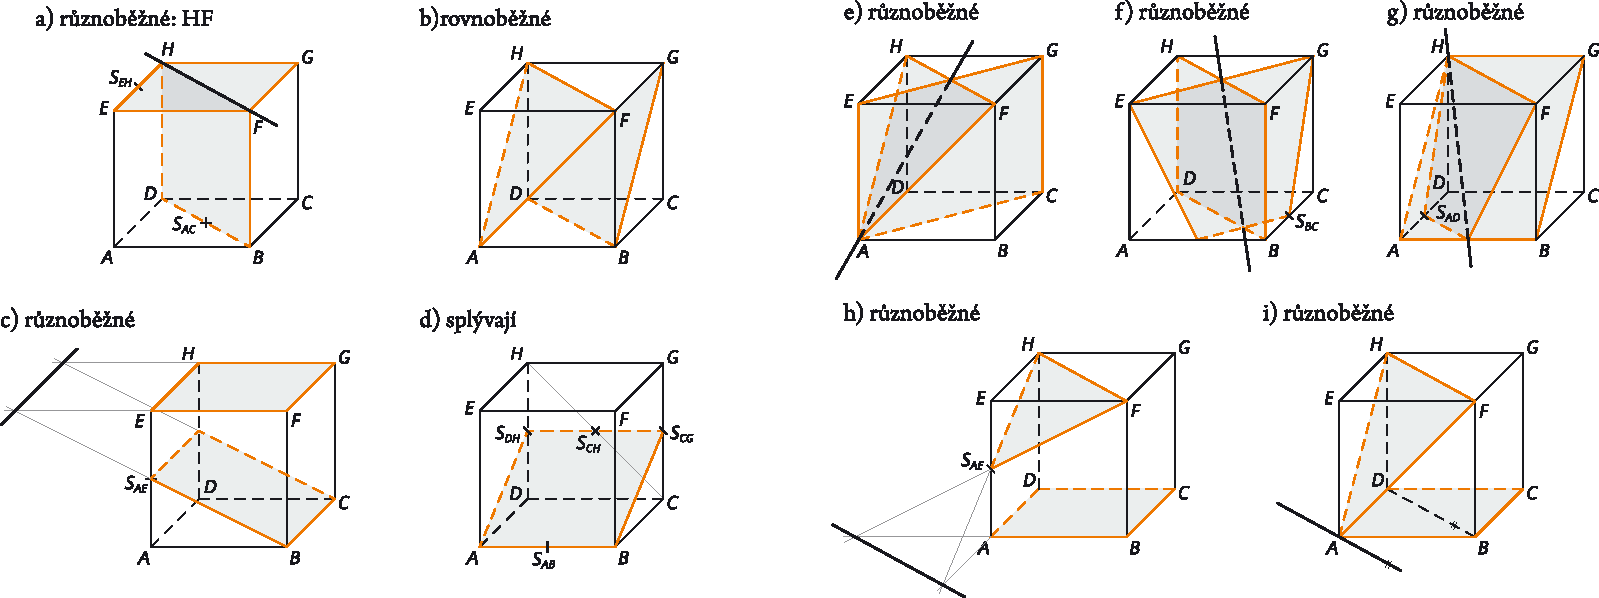
\includegraphics[width=\hsize]{vysl_prusecnice.pdf}\]}
\end{uloha}

\begin{uloha}
Mikrometeorit letící po přímce $MN$ narušil plášť krychle $ABCDEFGH$; zjistěte (konstrukčně), v jakých bodech to bylo.
\[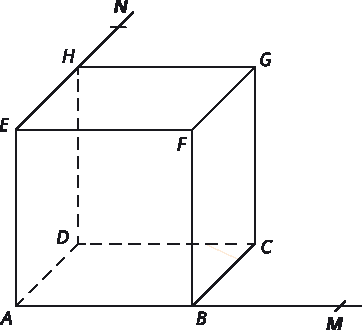
\includegraphics{meteorit.pdf}\]
\vyslplain{\[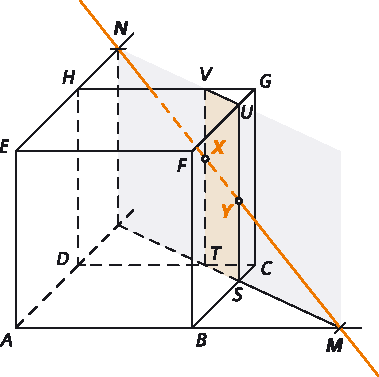
\includegraphics{meteorit_res.pdf}\]}
\end{uloha}


\newpage
\parindent=0pt
\parskip=\smallskipamount
\def\printvysl#1#2{\textbf{#1.}\ #2\par}
\vysld


\end{document}